%--------Modelo Estructural del Proceso de Infraestructura------------------%
\section{Modelo Estructural de Gestión de Infraestructura}
	%En la figura \ref{fig:infraestructuraDC} se muestra la estructura de información que manejará el \refElem{Calmecac} para llevar a cabo la gestión de unidades académicas, edificios y espacios.

\begin{figure}[hbtp!]
	\begin{center}
%				\fbox{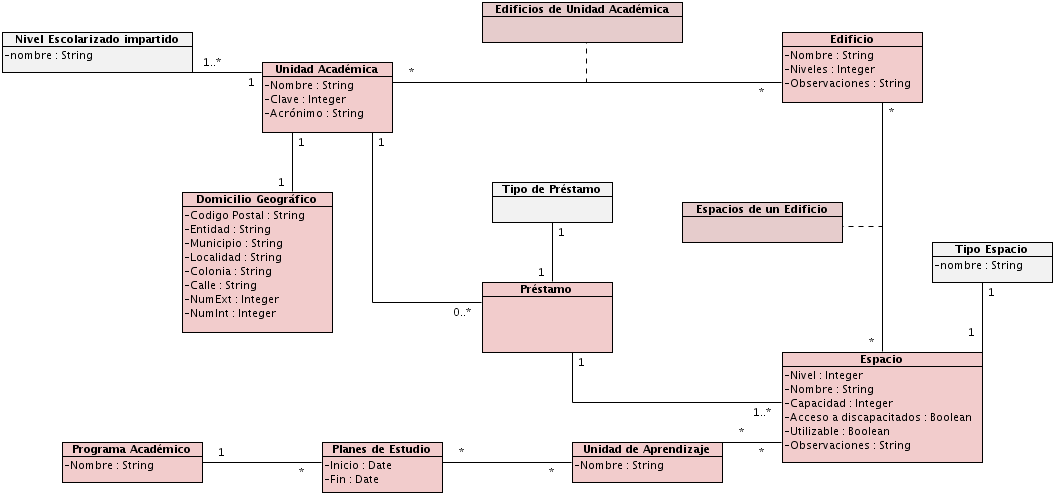
\includegraphics[width=\textwidth]{negocio/images/Modelodeinformacion_Procesodeinfraestructura_version_dos}}
%		\caption{Diagrama de Clases de Infraestructura}
%		\label{fig:infraestructuraDC}
	\end{center}
\end{figure}

%----------------------Entidades-------------------------------------------%

%=====Unidad Académica=====%
%\begin{cdtEntidad}{unidadAcademica}{Unidad Académica}
%	\brAttr{nombre}{Nombre}{Frase}{Es el nombre asignado a una unidad académica de acuerdo a los programas académicos que se imparten en ella}{\datRequerido}
%	\brAttr{clave}{Clave}{Entero}{Es la clave con la que una unidad académica puede ser identificada de otras}{\datRequerido}
%	\brAttr{acronimo}{Acrónimo}{Palabra}{Son las siglas con las que se pueden identificar las diferentes unidades académicas}{\datRequerido}
%	%----------------------------------
%	\cdtEntityRelSection
%	\brRel{\brRelAgregation}{\refElem{nivelEscolarizadoImpartido}}{Una \refElem{unidadAcademica} tiene  al menos un \refElem{nivelEscolarizadoImpartido}}
%	\brRel{\brRelComposition}{\refElem{domicilioGeografico}}{Una \refElem{unidadAcademica} reside en un \refElem{domicilioGeografico}}
%	\brRel{\brRelComposition}{\refElem{edificio}}{Una \refElem{unidadAcademica} tiene \refElem{edificio}}
%\end{cdtEntidad}


